\section{Design}\label{chapter:design}
\subsection{Generator}
The generator resides in the \texttt{de.hs\_rm.cs.vs.dsm.flow} plug-in project 
in the package \texttt{de.hs\-\_rm.\-cs.vs.dsm.flow.generator} and consists of 
two parts. The first part is a script written in the Xtend \cite{xtend} language 
which controls the transformation process of the query language to the target 
platform. It is the main entry point for the customization of the code 
generation process of the query language. The Xtend intepreter generates 
Java interfaces and classes which are stored in the \texttt{src-gen/} directory
in the same project and package. The second part of the generator are a set of
classes which are used for the target platform representation of code written in
the query language. Figure \ref{fig:generator} depicts the corresponding classes
and their relation. The figure omits method and attribute details which are 
described later in that section.
\begin{figure}[htpb]
  \centering
  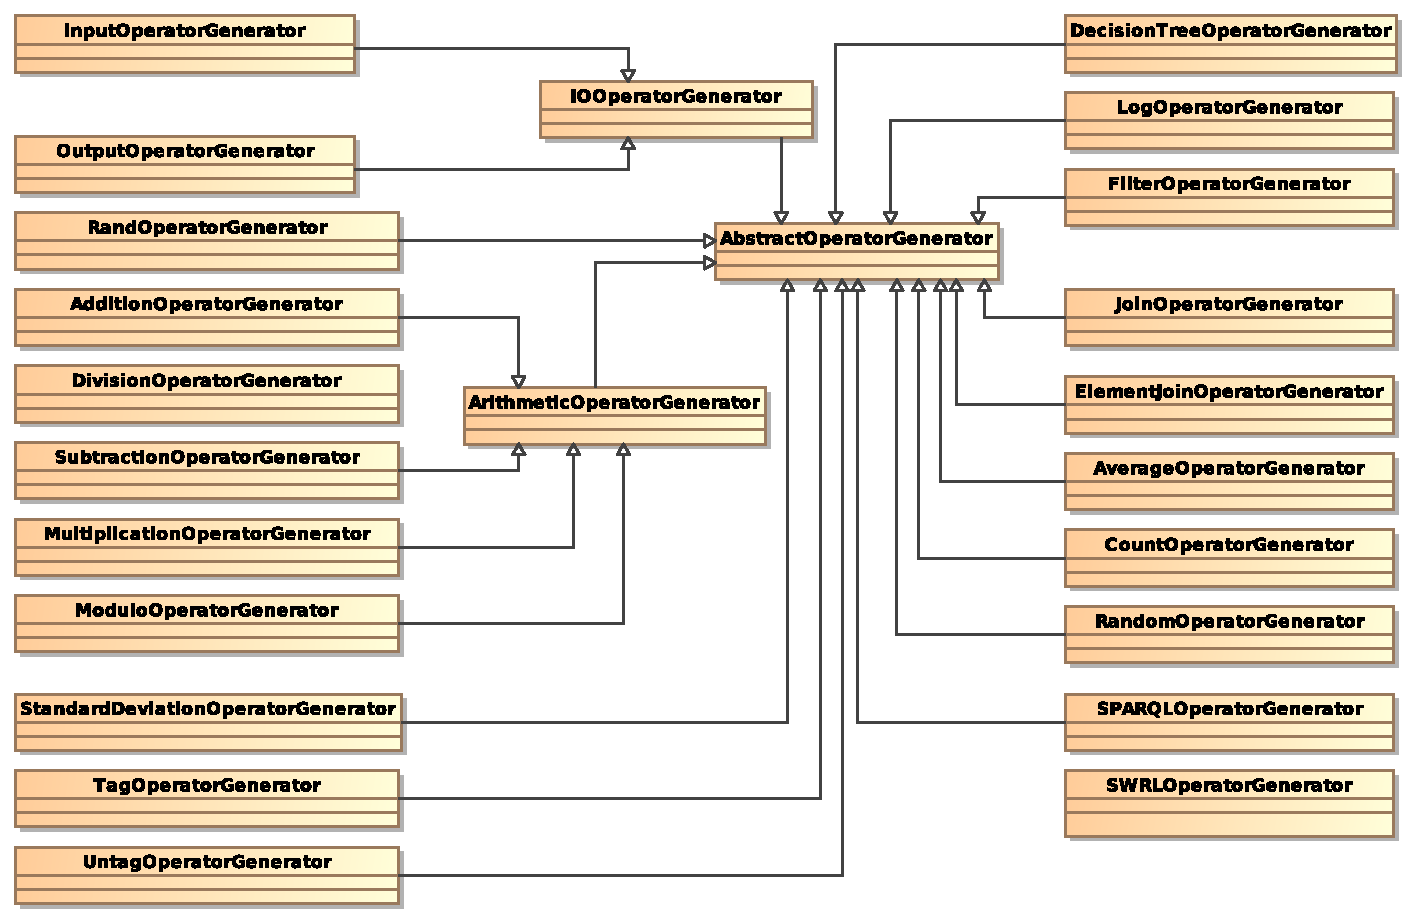
\includegraphics[width=1.0\textwidth]{figures/overview}
  \caption{\emph{Overview of classes which are used in code generation}}
  \label{fig:generator}
\end{figure}
Every operator of the query language is transformed into a set of LUA 
statements. The LUA script typically consists of statements for the 
initializiation of the framework, initialization and parameterization of 
operators, interconnecting operators, start and stop of operators. The class 
\texttt{AbstractOperatorGenerator} is depicted in figure 
\ref{fig:abstractoperatorgenerator} and provides abstract methods for the 
initialization (\texttt{initializeOperator()}), parameterization 
(\texttt{setOperatorProperties()}) and interconnection 
(\texttt{setOperatorConnection()}) of operators. Each operator generalizes from
\begin{figure}[htpb]
  \centering
  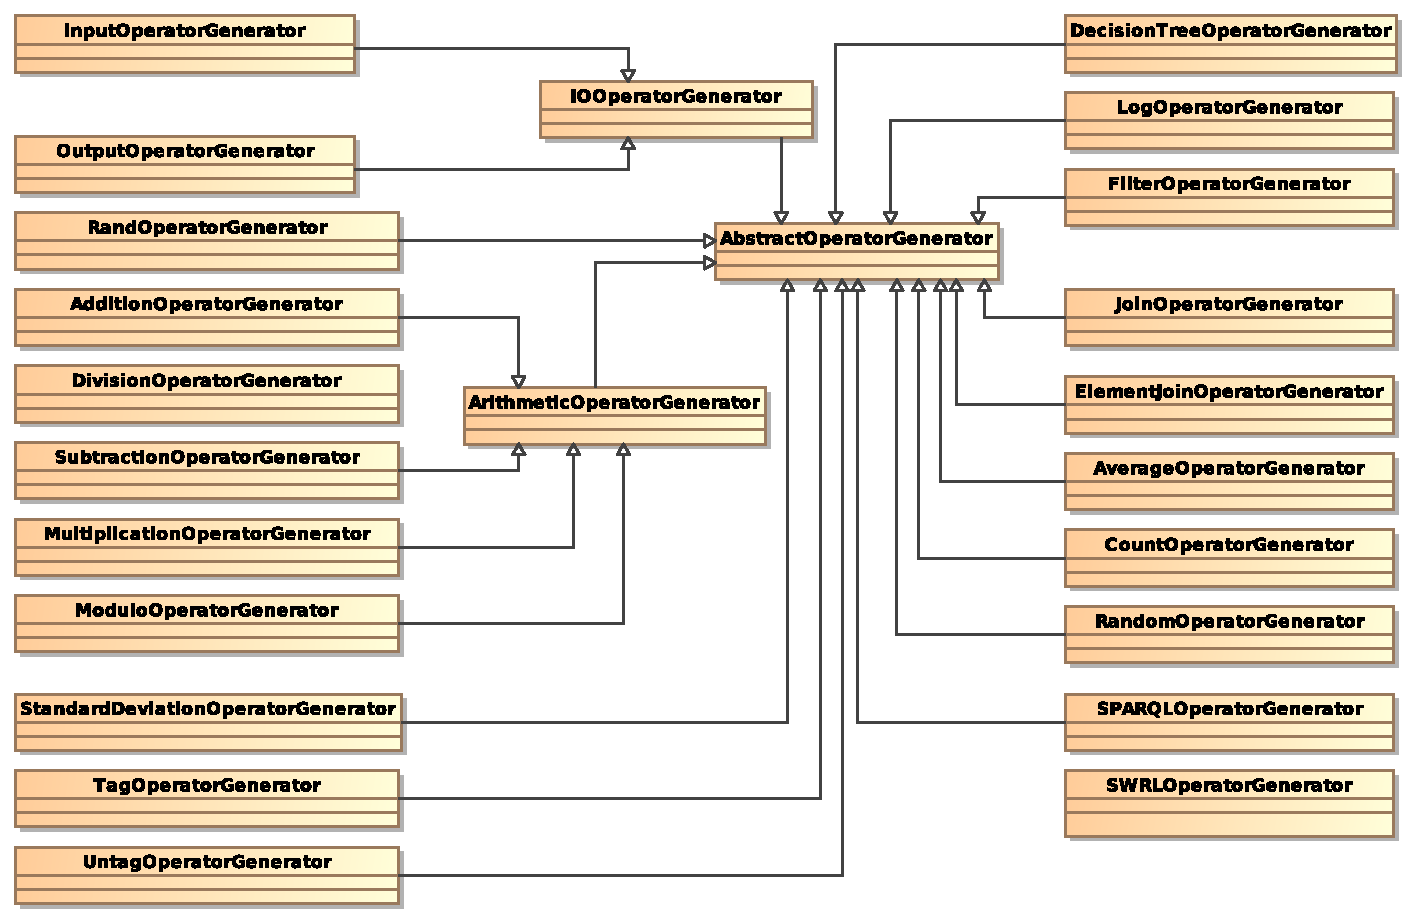
\includegraphics[width=0.8\textwidth]{figures/overview}
  \caption{\emph{UML class diagram of \texttt{AbstractOperatorGenerator}}}
  \label{fig:abstractoperatorgenerator}
\end{figure}
class \texttt{AbstractOperatorGenerator} and overwrites the abstract methods.

\subsubsection{Arithmetic Operators}
Supported arithmetic operators are \texttt{add} 
(\texttt{AdditionOperatorGenerator}), \texttt{sub} 
(\texttt{Subtraction\-OperatorGenerator}), \texttt{mult} 
(\texttt{MultiplicationOperatorGenerator}), \texttt{div} 
(\texttt{DivisionOperator\-Generator}) and \texttt{mod} 
(\texttt{ModuloOperatorGenerator}). Each operator inherits from class 
\texttt{Arithm\-eticperatorGenerator} which itself inherits from class
\texttt{AbstractOperatorGenerator}. Arithmetic operators are transformed to a
operator of type \texttt{Math}. The type of the arithmetic operation is set
as an attribute in LUA.

\subsubsection{Analysis Operators}
Analysis operatores are \texttt{avg} (\texttt{AverageOperatorGenerator}), 
\texttt{std} (\texttt{StandardDeviationOperatorGenerator}) and \texttt{count}
(\texttt{CountOperatorGenerator}).

\subsubsection{Structural Operators}

\subsubsection{Knowledge Operators}

\subsubsection{System Operators}
System operators are \texttt{in} (\texttt{InputOperatorGenerator}), 
\texttt{out} (\texttt{OutputOperatorGenerator}) and \texttt{log} 
(\texttt{LogOperatorGenerator}). The generators for the \texttt{in} and 
\texttt{out} operator are inheriting from a class \texttt{IOOperatorGenerator}.
The class transforms internationalized resource identifiers (IRI) to the 
corresponding LUA code. The corresponding UML class diagram is depicted in
figure \ref{fig:iooperatorgenerator} 
\begin{figure}[htpb]
  \centering
  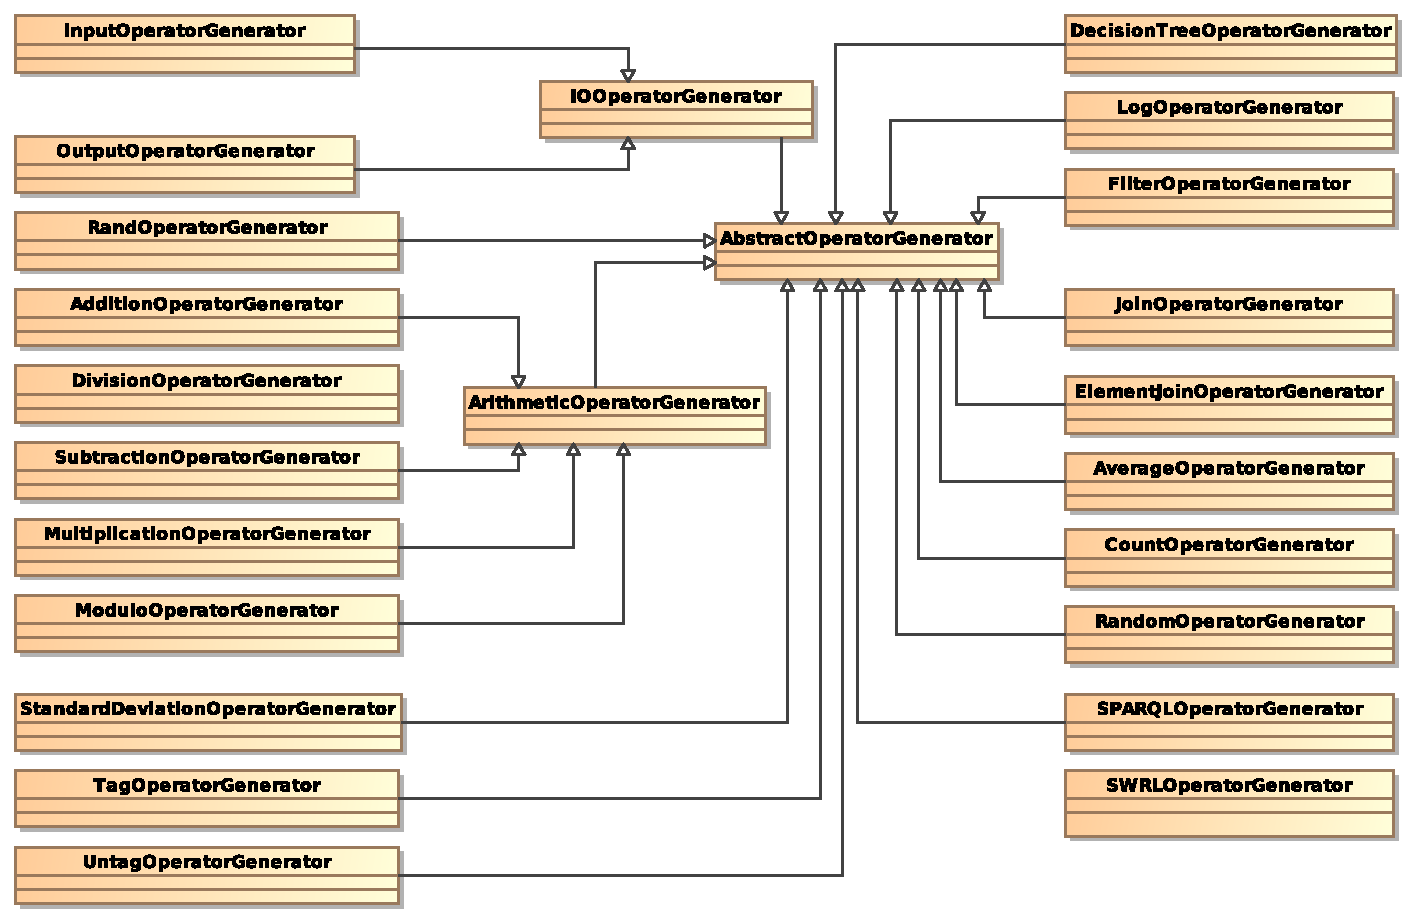
\includegraphics[width=0.8\textwidth]{figures/overview}
  \caption{\emph{UML class diagram of \texttt{IOOperatorGenerator}}}
  \label{fig:iooperatorgenerator}
\end{figure}
